\chapter{Results and Discussion}
\label{ch:results}

\section{Evaluation Protocol}
\label{sec:protocol}
All headline results use the following protocol, designed to match how a team would use the predictions.
\begin{itemize}
\item \textbf{Walk-forward folds.} Builds are sorted by trigger time and split into 10 equal chronological folds. Fold $k$ is tested after training on folds $1,\dots,k-1$, and the test folds are 6--10. On Travis~CI every design choice for \tierE\ was made on fold~6 alone; folds 7--10 were then scored once.
\item \textbf{Metric.} The primary metric is \emph{macro within-repository AUC}: the AUC computed within each repository that has both passes and failures in the test fold, averaged over repositories. 0.5 means random ranking and 1.0 perfect ranking. We also report \emph{recall@15\%}, the share of a repository's failures found when it reviews its riskiest 15\% of builds.
\item \textbf{Uncertainty.} Differences between models are paired by repository, and 95\% confidence intervals come from 1,000 bootstrap resamples of repositories~\cite{efron1993introduction}.
\item \textbf{Controls.} When training labels are randomly shuffled, the ranker drops to 0.48--0.50 within-repository AUC, as it should, which confirms that no label leaks into the features.
\item \textbf{Pre-registration.} Each GitHub Actions test followed a written protocol, fingerprinted (SHA-256) and committed before its data was collected~\cite{nosek2018preregistration}. Its decision rule was fixed in advance: \emph{confirms} if the mean gain over folds 6--10 is positive and at least 4 of 5 fold confidence intervals exclude zero; \emph{inconclusive} if the mean gain is positive otherwise; \emph{does not replicate} if it is not positive.
\end{itemize}

\section{How Much the Usual Evaluation Overstates Results}
\label{sec:leakage}
Table~\ref{tab:dev} and Fig~\ref{fig:modelcmp} compare the six classifiers in the way most studies do: a random 80/20 split of a 200,000-row sample. On this split, Random Forest, XGBoost and the stacking ensemble look strong (AUC 0.90--0.91, F1 about 0.73), while Decision Tree and SVM trail.

\begin{table}[H]
\centering
\caption{Development comparison of classifiers (random split; reference only)}
\label{tab:dev}
\begin{tabular}{|l|r|r|r|r|r|}
\hline
\textbf{Model} & \textbf{Accuracy} & \textbf{Precision} & \textbf{Recall} & \textbf{F1} & \textbf{AUC}\\ \hline
Stacking (RF + XGB + LGBM) & 0.899 & \textbf{0.831} & 0.653 & \textbf{0.731} & \textbf{0.912}\\ \hline
Random Forest & 0.889 & 0.749 & 0.714 & 0.731 & 0.908\\ \hline
XGBoost & 0.889 & 0.752 & 0.709 & 0.730 & 0.900\\ \hline
LightGBM & 0.877 & 0.699 & 0.729 & 0.714 & 0.898\\ \hline
Decision Tree & 0.769 & 0.469 & \textbf{0.741} & 0.575 & 0.825\\ \hline
SVM & 0.758 & 0.447 & 0.623 & 0.520 & 0.772\\ \hline
\end{tabular}
\end{table}

\begin{figure}[H]
\centering
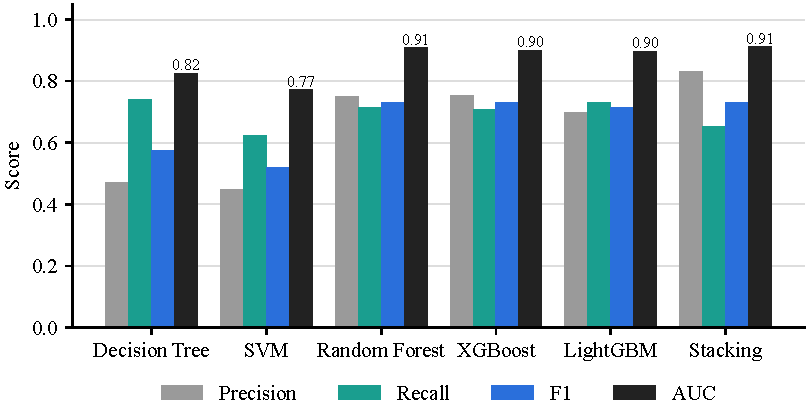
\includegraphics[width=0.95\textwidth]{model_comparison.pdf}
\caption{Development comparison of six classifiers on a random split (reference only)}
\label{fig:modelcmp}
\end{figure}

These numbers do \emph{not} describe real use. A random split lets a model learn each repository's future failure rate from builds that come later in time. Table~\ref{tab:leak} and Fig~\ref{fig:leakage} show the same task as the evaluation becomes progressively stricter:
\begin{itemize}
\item On a random split, adding fields from the build log lifts AUC from 0.690 to 0.896. Those fields are not available before a build runs, and the availability registry now blocks them.
\item Without leaky fields, the random-split AUC of 0.91 falls to 0.82 on a chronological split.
\item It falls to \textbf{0.63} when measured within each repository at the build level, which is how a team would experience it.
\end{itemize}
The rest of this chapter reports only this strict setting.

\begin{table}[H]
\centering
\caption{The same task under progressively stricter evaluation (Travis~CI)}
\label{tab:leak}
\begin{tabular}{|p{11cm}|r|}
\hline
\textbf{Setup} & \textbf{AUC}\\ \hline
Random split, 31 features including post-build log fields (leaky) & 0.896\\ \hline
Random split, 13 strict pre-build features & 0.690\\ \hline
Random split, 39 features with repository history (stacking) & 0.912\\ \hline
Chronological split, job level, pooled over repositories (Random Forest) & 0.821\\ \hline
Walk-forward, build level, \emph{within-repository} (\tierC\ Random Forest) & 0.628\\ \hline
Walk-forward, build level, \emph{within-repository} (\tierE, this project) & \textbf{0.698}\\ \hline
\end{tabular}
\end{table}

\begin{figure}[H]
\centering
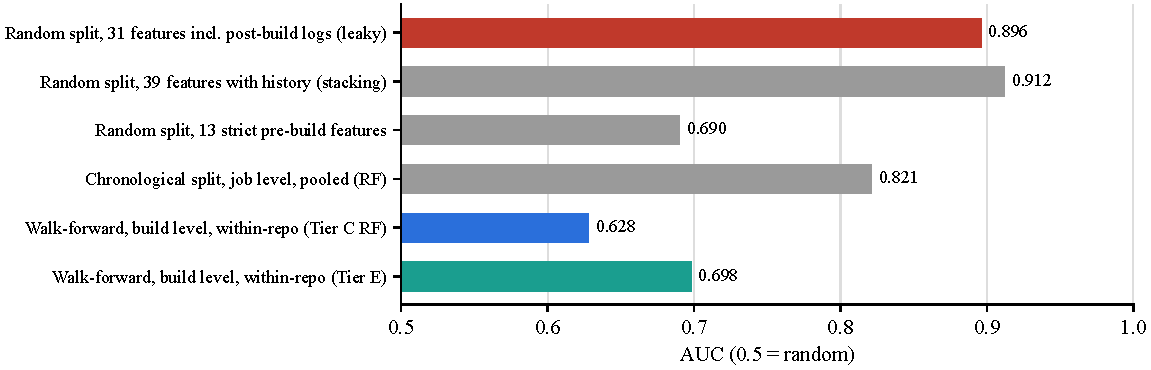
\includegraphics[width=0.95\textwidth]{leakage_ladder.pdf}
\caption{AUC under progressively stricter evaluation. Red: uses leaked post-build fields. Blue and teal: the strict protocol used for all results that follow.}
\label{fig:leakage}
\end{figure}

\section{Results on Travis CI}
\label{sec:travis}
Fig~\ref{fig:main} summarizes every evaluation. On Travis~CI, \tierE\ raises macro within-repository AUC from 0.628 to \textbf{0.698} (+0.070), and every confirmation fold's 95\% confidence interval is above zero. The per-fold gains are +0.068, +0.067, +0.070 and +0.074. Recall@15\% within each repository improves by +0.068.

\begin{figure}[H]
\centering
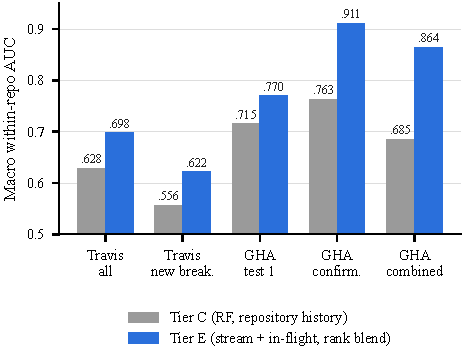
\includegraphics[width=0.78\textwidth]{main_results.pdf}
\caption{Macro within-repository AUC of \tierC\ (Random Forest with repository history) and \tierE\ across all evaluations (test folds; outcomes known as soon as builds finish)}
\label{fig:main}
\end{figure}

\minorhead{Robustness to reporting delays}
Table~\ref{tab:travis} repeats the evaluation with outcomes withheld for an extra 1 or 6 hours. Unlike a pure ``it failed last time'' effect, the gain \emph{grows} as outcomes are withheld longer (Fig~\ref{fig:buffer}). The in-flight features, such as whether the previous build is still running, stay informative when recent outcomes are not yet known.

\begin{table}[H]
\centering
\caption{Travis~CI results by finish buffer (folds 7--10). Every fold's 95\% CI for the gain is above zero.}
\label{tab:travis}
\begin{tabular}{|c|r|r|r|}
\hline
\textbf{Finish buffer} & \textbf{\tierC\ Random Forest} & \textbf{\tierE} & \textbf{Gain}\\ \hline
0 h & 0.628 & \textbf{0.698} & +0.070\\ \hline
1 h & 0.600 & \textbf{0.681} & +0.081\\ \hline
6 h & 0.585 & \textbf{0.672} & +0.087\\ \hline
\end{tabular}
\end{table}

\begin{figure}[H]
\centering
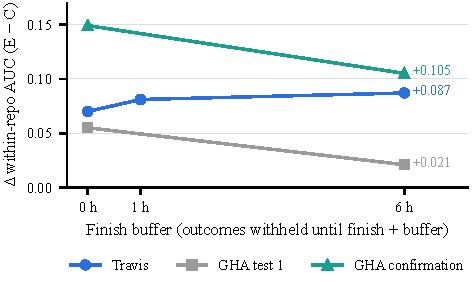
\includegraphics[width=0.72\textwidth]{finish_buffer.pdf}
\caption{Gain of \tierE\ over \tierC\ as outcomes are withheld longer}
\label{fig:buffer}
\end{figure}

\minorhead{What drives the gain}
Table~\ref{tab:attr} separates the ingredients.
\begin{itemize}
\item The learning-to-rank objective is the largest single lever on Travis~CI: it is worth +0.031 on \tierC\ features alone.
\item Stream and in-flight features add about +0.03 more.
\item Build-matrix size, the number of jobs, adds only about 0.003, so the deployed variant omits it.
\end{itemize}
The ranker trades overall (pooled) AUC for within-repository ordering. Teams that need a pooled ranking across repositories should use the binary \tierE\ model, which beats \tierC\ on both measures.

\begin{table}[H]
\centering
\caption{Attribution of the \tierE\ gain on Travis~CI (folds 7--10)}
\label{tab:attr}
\begin{tabular}{|l|r|r|}
\hline
\textbf{Variant} & \textbf{Within-repo AUC} & \textbf{Pooled AUC}\\ \hline
\tierC, Random Forest & 0.628 & 0.856\\ \hline
\tierC, binary LightGBM & 0.633 & --\\ \hline
\tierC, LightGBM ranker & 0.664 & --\\ \hline
\tierE, binary LightGBM & 0.652 & \textbf{0.881}\\ \hline
\tierE, LightGBM ranker & 0.696 & --\\ \hline
\tierE, blend & \textbf{0.698} & 0.828\\ \hline
\tierE, blend without job counts & 0.695 & 0.826\\ \hline
\end{tabular}
\end{table}

\section{New Breakages}
\label{sec:newbreak}
Much of the signal comes from branches or pull requests that are already failing: 55\% of failures occur on streams whose last known outcome was a failure. To check that the model does more than repeat the last outcome, the saved predictions were rescored on \emph{new breakages}, builds whose previous build on the same stream passed. These are 25\% of failures, and such builds fail only 6.6\% of the time.
\begin{itemize}
\item On new breakages, the repository's recent failure rate is at chance (0.504) and \tierC\ scores 0.556.
\item \tierE\ scores \textbf{0.622}, a gain of +0.066, as large as on all builds, with every fold's interval above zero.
\item With a 15\% review budget, \tierE\ catches 30\% of new breakages (lift 1.78$\times$) against 24\% for \tierC.
\end{itemize}
The honest headline for \emph{fresh} breakages is therefore about 0.62, not 0.70. This analysis was carried out after the main results (post hoc).

\section{Pre-Registered Tests on GitHub Actions}
\label{sec:gha}
The frozen recipe was tested on GitHub Actions, a different CI platform, without any changes.

\minorhead{Test 1 (30 repositories): inconclusive}
\tierE\ scored 0.770 against 0.715 (+0.055) and was ahead in all five folds. However, only 3 of 5 fold intervals excluded zero, and the rule required 4, so the pre-registered verdict is \emph{inconclusive} (Table~\ref{tab:gha1}). Recall@15\% was 0.48 against 0.37.

\begin{table}[H]
\centering
\caption{First GitHub Actions test (30 repositories, folds 6--10)}
\label{tab:gha1}
\begin{tabular}{|l|r|r|r|c|}
\hline
\textbf{Setting} & \textbf{\tierC} & \textbf{\tierE} & \textbf{Gain} & \textbf{Folds clearly ahead}\\ \hline
All runs (primary) & 0.715 & \textbf{0.770} & +0.055 & 3/5\\ \hline
Label-validity check & 0.703 & 0.754 & +0.051 & 3/5\\ \hline
New breakages & 0.645 & 0.695 & +0.050 & 0/5\\ \hline
All runs, 6 h buffer & 0.698 & 0.718 & +0.021 & 0/5\\ \hline
\end{tabular}
\end{table}

\minorhead{Confirmation (30 new repositories): confirms}
A second protocol was fixed before collecting data from 30 repositories never used before. Here \tierE\ scored \textbf{0.911} against 0.763 (+0.149). All five fold intervals exclude zero, and the smallest lower bound is +0.090 (Fig~\ref{fig:folds}, Table~\ref{tab:confirm}). Recall@15\% rose from 0.31 to 0.43, and \tierE\ beat \tierC\ in all 24 test repositories. A secondary analysis on both datasets together (60 repositories) gave +0.179, again 5 of 5 folds.

\begin{figure}[H]
\centering
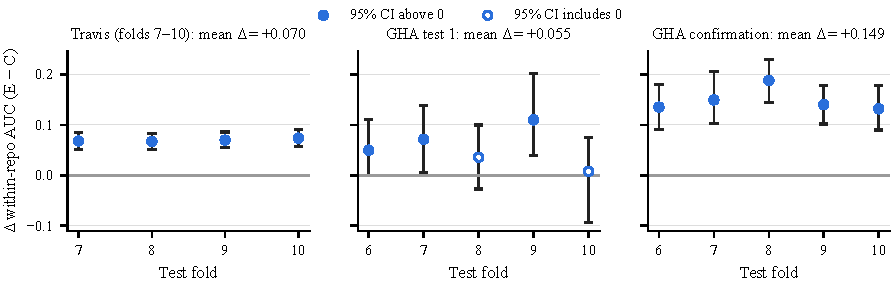
\includegraphics[width=\textwidth]{fold_deltas.pdf}
\caption{Per-fold gain of \tierE\ over \tierC\ with 95\% confidence intervals. Filled markers: the interval excludes zero.}
\label{fig:folds}
\end{figure}

\begin{table}[H]
\centering
\caption{GitHub Actions confirmation test (30 new repositories, folds 6--10)}
\label{tab:confirm}
\begin{tabular}{|l|r|r|r|c|}
\hline
\textbf{Setting} & \textbf{\tierC} & \textbf{\tierE} & \textbf{Gain} & \textbf{Folds clearly ahead}\\ \hline
All runs (primary) & 0.763 & \textbf{0.911} & +0.149 & 5/5\\ \hline
Label-validity check & 0.765 & 0.911 & +0.147 & 5/5\\ \hline
New breakages & 0.642 & 0.683 & +0.041 & 2/5\\ \hline
All runs, 6 h buffer & 0.741 & 0.846 & +0.105 & 5/5\\ \hline
New breakages, 6 h buffer & 0.637 & 0.634 & $-$0.004 & 0/5\\ \hline
Combined, 60 repositories & 0.685 & 0.864 & +0.179 & 5/5\\ \hline
\end{tabular}
\end{table}

\minorhead{Is it only ``it failed last time''?}
The confirmation gain is almost three times the first test's, and failures were three times as common. We therefore checked a naive rule that predicts failure when the stream's previous finished run failed. It scores only about 0.72, below \tierC\ (Fig~\ref{fig:persist}), and the gain per repository is unrelated to the repository's failure rate (correlation 0.03). This check was exploratory.

\begin{figure}[H]
\centering
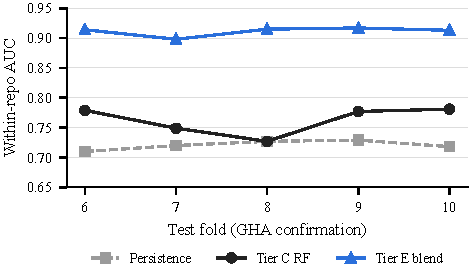
\includegraphics[width=0.75\textwidth]{persistence.pdf}
\caption{Confirmation test: \tierE\ against \tierC\ and a naive persistence rule}
\label{fig:persist}
\end{figure}

\minorhead{Discussion}
On GitHub Actions, the stream and in-flight features carry the gain; the ranking objective alone adds only +0.010 (test~1) and +0.042 (confirmation). Most runs finish within an hour, so the very recent outcome of the same stream is the key signal. Withholding it for 6 hours removes most of the gain on new breakages. The size of the gain varies by project (+0.055 to +0.149), but its direction is consistent across Travis~CI and both GitHub Actions tests.

\section{Deployed Model and Alert Policy}
\label{sec:alerts}
The deployed model was trained on folds 1--9 of the 146,556 GitHub Actions runs. Table~\ref{tab:holdout} shows its results on the newest 10\%. To estimate how it performs on a repository it has never seen, the holdout was rescored with all workflow identities hidden; it still reaches 0.893.

\begin{table}[H]
\centering
\caption{Deployed model on its holdout (newest 10\% of GitHub Actions runs, 20 repositories)}
\label{tab:holdout}
\begin{tabular}{|l|r|}
\hline
\textbf{Measure} & \textbf{Value}\\ \hline
Within-repository AUC & 0.913\\ \hline
Within-repository AUC, repository never seen & 0.893\\ \hline
Within-repository recall at a 15\% review budget & 43.3\%\\ \hline
Pooled AUC & 0.936\\ \hline
Failure rate of the holdout & 36.3\%\\ \hline
\end{tabular}
\end{table}

\minorhead{Alert policy}
A single global threshold set to flag 15\% of the holdout sits at 0.94, because that holdout fails often. It flags between 3\% and 51\% of a repository's runs. The per-repository budget instead flags each repository's riskiest 15\% of recent runs (Section~\ref{sec:deployed}). Replayed in time order on the holdout, each repository flags 11--22\% of its runs, and the share of a repository's failures caught rises from 34\% to 41\%, close to the 43\% measured in hindsight (Table~\ref{tab:alert}, Fig~\ref{fig:alert}). Pooled precision is lower only because the global threshold spends almost all its alerts on the repositories that fail most.

\begin{table}[H]
\centering
\caption{Alert policies compared on the deployed model's holdout}
\label{tab:alert}
\begin{tabular}{|l|r|r|}
\hline
\textbf{Measure} & \textbf{Global threshold (0.94)} & \textbf{Per-repository budget}\\ \hline
Runs flagged per repository & 3--51\% & 11--22\%\\ \hline
Failures caught per repository (mean) & 34\% & \textbf{41\%}\\ \hline
Share of alerts that were failures & 0.97 & 0.80\\ \hline
\end{tabular}
\end{table}

\begin{figure}[H]
\centering
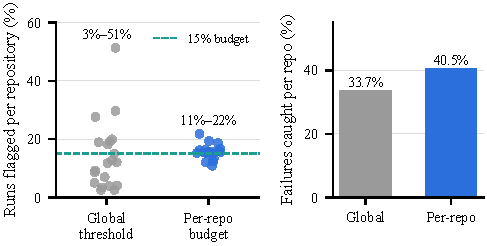
\includegraphics[width=0.75\textwidth]{alert_policy.pdf}
\caption{Global threshold vs.\ per-repository alert budget: share of each repository's runs flagged (left) and failures caught (right)}
\label{fig:alert}
\end{figure}

\minorhead{Public demonstration}
In the public demonstration, the 450 replayed runs are scored with the history the system builds up live, starting empty. Within-repository AUCs are 0.80 (freeCodeCamp), 0.95 (bootstrap) and 0.74 (yt-dlp), close to the research evaluation of the same runs (0.78, 0.97 and 0.79). The model-evidence panel of the dashboard (Fig~\ref{fig:dash_models}) presents these research results alongside the deployed model's holdout statistics.

\begin{figure}[H]
\centering
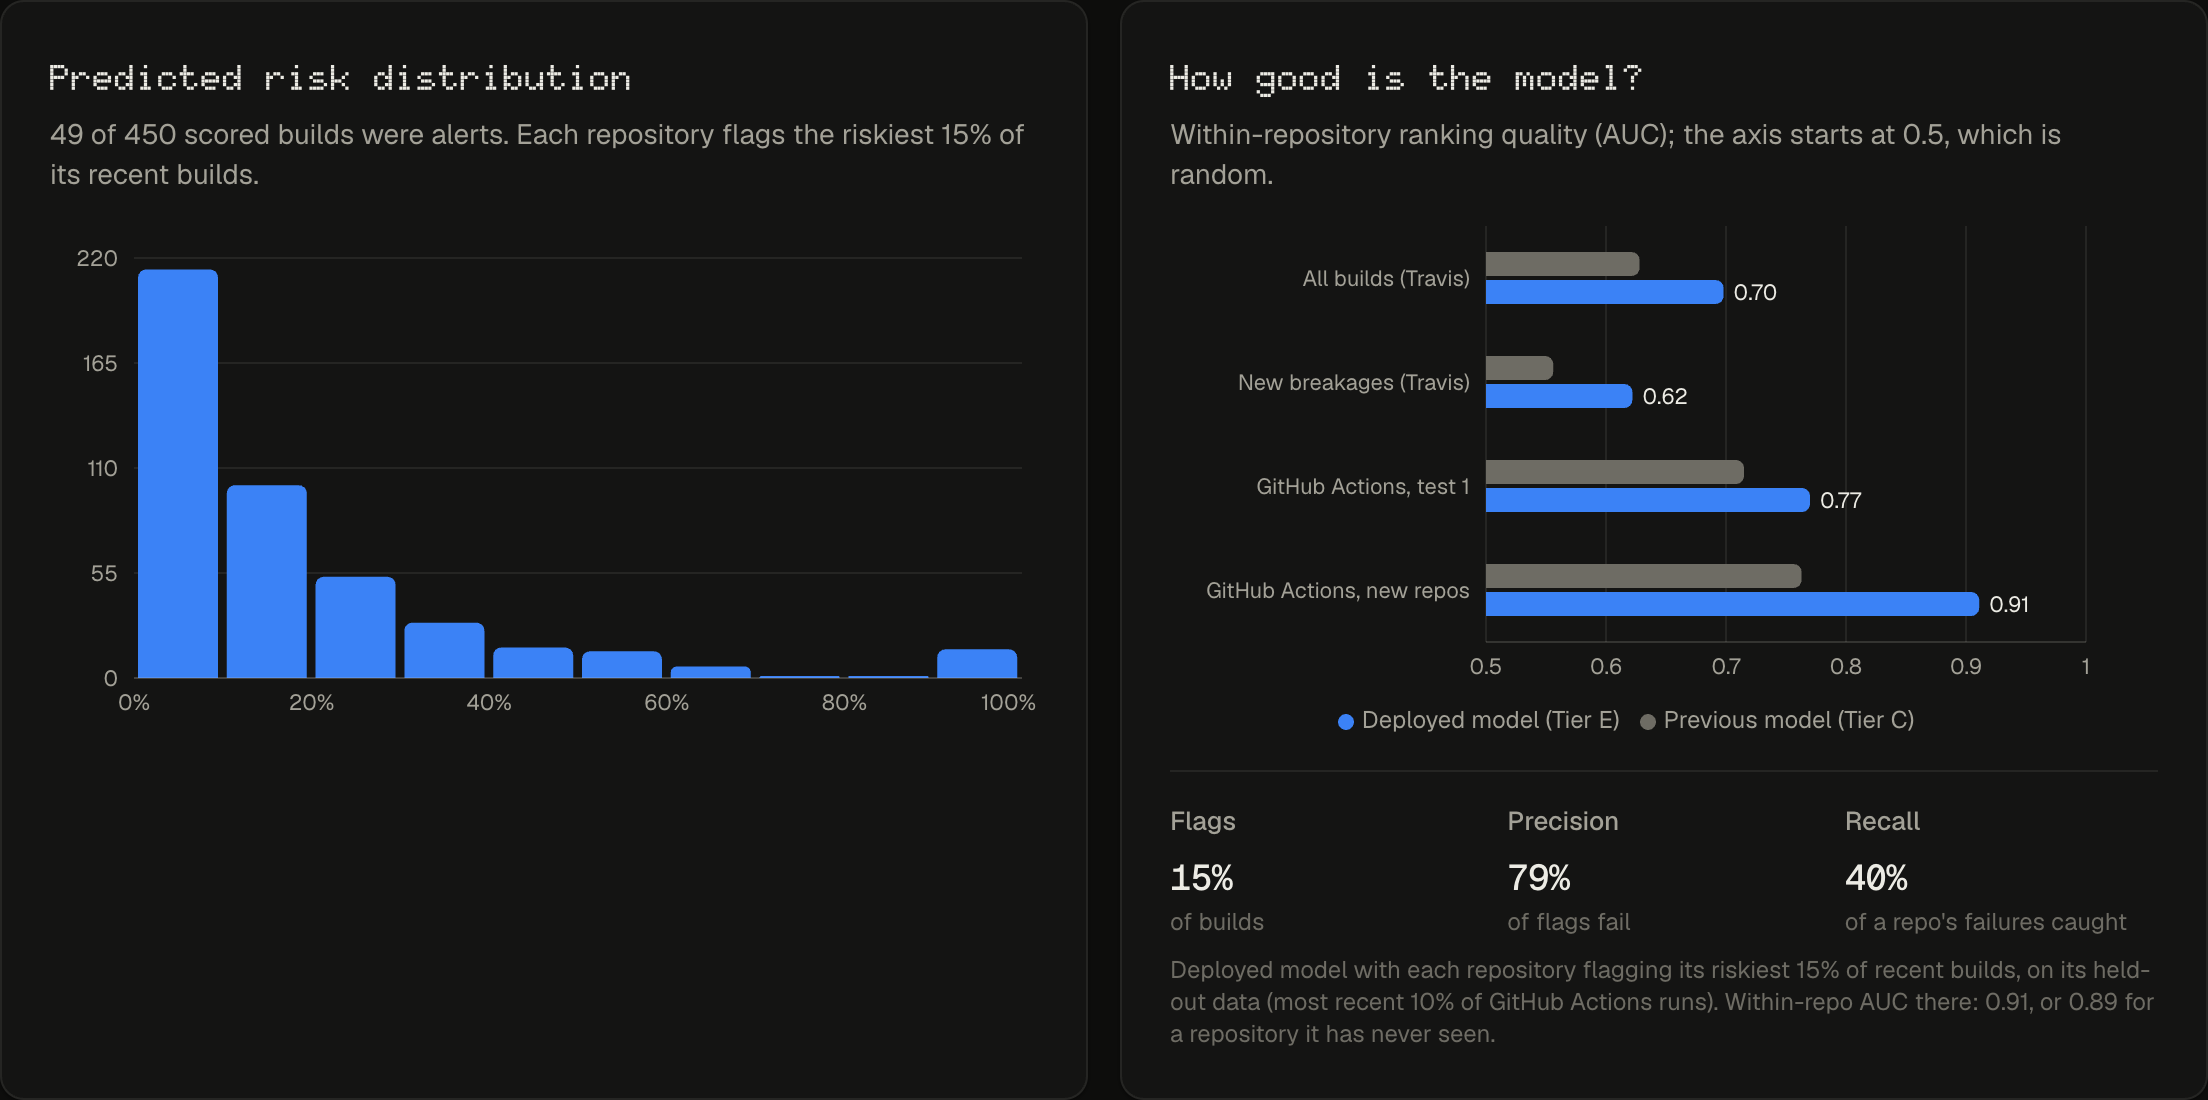
\includegraphics[width=\textwidth]{dashboard_models.png}
\caption{Dashboard: risk distribution of the 450 demonstration runs (49 alerts under the per-repository budget) and the model-evidence panel}
\label{fig:dash_models}
\end{figure}

\section{Negative Results}
\label{sec:negative}
\begin{itemize}
\item \textbf{Repository-level streaks hurt.} Adding repository-level failure streaks and time gaps to \tierC\ \emph{reduced} within-repository AUC by 0.019, significantly in 4 of 5 folds. Streaks that mix all of a repository's branches are noise; per-stream history is the version of this idea that helps.
\item \textbf{Anomaly flag.} Builds flagged as anomalous by Isolation Forest did not fail more often, so the flag is kept as a diagnostic rather than presented as a risk signal.
\end{itemize}

\section{Threats to Validity}
\label{sec:threats}
\begin{itemize}
\item \textbf{Post-hoc analyses.} The new-breakage analysis and the persistence check were carried out after the main results. On Travis~CI fold~6 was used for development, so only folds 7--10 are confirmatory.
\item \textbf{Approximate finish times.} Finish times on Travis~CI are derived from job durations, with a fallback for missing ones.
\item \textbf{Lost runs.} In the confirmation data, 4.6\% of runs were lost to unfetchable fork commits, and these runs failed more often (38.5\% vs.\ 28.2\%).
\item \textbf{Selection.} Repositories come from popular open-source projects. Capping each repository at 4,000 runs left six of the busiest projects in training folds only.
\item \textbf{What the metric measures.} Within-repository AUC measures ranking, not calibrated probability. Recall at a 15\% budget assumes that teams review a fixed share of builds.
\end{itemize}
